\documentclass[../../thesis.tex]{subfiles}

\begin{document}

\TODO{Introduce the section, what we think and the philosophy of presenting material in such a way.}


\section{Information theoretic/basic stats used in evaluation}

- mutual information

- entropy

- perplexity

- KL-divergence

\section{General time series stuff}
- short-time-fourier transform etc.

\section{Neural Network}

Ref is \cite{deeplearningbook} chapter 6. ISLRv2 chapter 10

\textit{Feedforward neural network}, \textit{artificial neural network}, \textit{multilayer perceptron} or simply \textit{neural network} is a fundemental model in machine learning, and more specifically in \textit{deep learning}. \TODO{History}

A neural network takes in a vector of $x \in \mathbb{R}^n$ variables and builds a nonlinear function $f(x)$ to predict the response $y\in \mathbb{R}^m$. In particular a neural network maps an input vector $x$ to an output vector $y$ through a series of non-linear functions of linear combinations of the input. This particular structure, presented in figure [fig of nn here] is what distinguishes neural networks from other nonlinear prediction models. The variables $x = [x_1,...,x_n]$ constitutes the units of \textit{input layer}. The intermediate layers are called the \textit{hidden layers}, and the final mapping to $y$ is called the \textit{output layer}.

A neural network is parameterized by a set of \textit{weight} matrices $W_i$ and \textit{bias} vectors $b_i$, together with a specified non-linear \textit{activation function} $\sigma$. Written out a $K$ layered neural network is given by 
\[ 
f(x) = f_o \circ f_K \circ \ldots \circ f_1(x),
\]
where 
$$f_i = \sigma(W_ix+b_i), \quad i \in \{1,...,K\},$$ 
and $f_o$ is the output layer whos form is application dependent. It is worth mentioning that $\sigma$ is applied pointwise.

Two of the most commonly used activation functions are $\text{Sigmoid}(x) = \tfrac{1}{1+\exp(-x)}$ and $\text{ReLU}(x) = \max(0,x)$.  

\TODO{Importance of activation functions. The role of ReLU in the development of modern ML}


\TODO{Sneak in something about universal approximation theorem}

\section{Convolutional Neural Network}
This section draws heavily on the presentation of convolutional networks in chapter 9 of \cite{deeplearningbook}.\\\\

A convolutional neural network (CNN) is a particular type of neural network that is developed to learn local features in the data. This local feature learning is enabled by the mathematical operation of convolution. 

In essence a CNN is a neural network where matrix multiplication is switched for convolution at least one of the layers \cite{deeplearningbook}. 

Some history: 1959 visual cortex cells. The Neocognitron 1980. CNN for MNIST Yann LeCun 1989- 1998. AlexNet: GPU training and popularization of deep neural nets.

Why was it introduced? 
Fully connected neural networks suffer badly from overfitting. Vanishing gradient / exploding gradient.

What problems did it solve?

\subsection{The convolution operation}

The convolution operation is an integral transform with extensive applications. It generalizes the notion of a moving weighted average. In mathematics it is ubiquitous because of its relationship with the Fourier transform.
\\\\
Let $f$ and $g$ be real valued functions, then their convolution is defined as
\begin{equation}
    (f*g)(t) = \int_{-\infty}^{\infty} f(\tau)g(t-\tau) d\tau
\end{equation}

The mathematical nuances of the exact criteria for the above integral to exist is outside the scope of this thesis, and not particularly relevant. But if $f$ and $g$ are integrable (in the Riemann or Lebesgue sense) then the convolution exists. As a rule of thumb, the convolution of $f$ and $g$ is as "smooth" as the smoothest of $f$ and $g$. It is worth mentioning that convolution is commutative, i.e that $f*g = g*f$, which can be seen by a simple change of variables. 
\\\\ 
As is typical for integral transforms, the function $g$ is referred to as the \textit{kernel}. In the context of convolutional networks the kernel consists of learnable parameters and the function $f$ is the \textit{input}. The output is sometimes referred to as the \textit{feature map} \cite{deeplearningbook}. In machine learning we handle discrete signals, represented as multidimensional arrays. As a result we must employ a discrete variation of the convolution operation. Let $I$ be the input and $K$ be the kernel, both discrete, then their convolution is defined as
\begin{equation}
    (I*K)[n] = \sum_{m=-\infty}^{\infty} I[m]K[n-m].
\end{equation}
In practice $I$ and $K$ typically has finite support, i.e they are zero for large positive and negative arguments, which circumvents any convergence problem.\\\\
Convolutions are naturally defined for higher dimensional functions, by component wise extension. For a two dimensional image $I$ and a kernel $K$ we calculate their convolution as 
\begin{equation}
    (I*K)[i,j] = \sum_{n=-\infty}^{\infty}\sum_{m=-\infty}^{\infty} I[n,m]K[i - n,j - m]. 
\end{equation}

\TODO{Figure of convolution}

- In applications the kernel dimensions are much smaller than the input dimensions. 

- Stride 

- Kernel dim and stride length determines downsample rate (reduction in size). 

- In a convolutional layer the kernel is learned such that the feature map is helpful for the training objective. 


Convolution in machine learning does not always correspond exactly to the mathematical definition of the operation, but rather to cross-correlation. The difference is just a sign flip in the kernel arguments. Operation is no longer commutative, but in practice this does not affect anything as the learned kernel parameters will be equivalent \cite{deeplearningbook}. Machine learning applications are focused on what works, rather than writing proofs. \\\\



"Convolution leverages three important ideas that can help improve ML systems: sparse interactions, parameter sharing and equivariant representations" \cite{deeplearningbook}.

\subsection{Pooling}
A pooling operation is applied as a down sample technique on feature maps in CNNs, replacing regions of the output with summary statistics. Two of the most common are max and average pooling, which replaces the region by its maximal or average value respectively. There are two hyperparameters for any pooling operation, the filter size, which determines the area of values to calculate the summary statistic, and stride length, which determines how the filter moves across the feature map. 

\begin{figure}[h]
    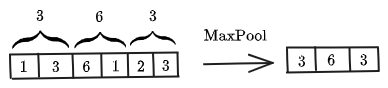
\includegraphics[scale=0.5]{MP_stride2}
    \centering    
    \caption{Max pooling of one dimensional array. Filter size: $2$, stride: $2$.}
\end{figure}
\begin{figure}[h]
    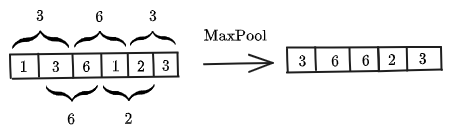
\includegraphics[scale=0.5]{MP_stride1}
    \centering    
    \caption{Max pooling of one dimensional array. Filter size: $2$, stride: $1$.}
\end{figure}

- Pooling assist in making the representations approximately invariant to small distortions of input. 

- Pooling is often essential in handling variable input size.

- 

\subsection{Architecture}
A typical layer in a convolutional network consists of three stages: 

Convolution: Hidden layer with regular matrix multiplication with weight matrix $W$ is switched out with convolution with kernel matrix $K$.

non-linear activation: Point wise nonlinearity, ReLU, sigmoid etc.

pooling layer: Max, average etc. pooling of feature map.





\subsection{Transposed Convolutional Networks}
Transposed convolution, also known as fractionally-strided convolution is a technique used to reverse the downsampling from convolutions. 




\section{Residual Neural Network}

Deep neural networks are hard to train. But we want deeper networks as the representations learned in deeper networks tend to be higher level/more abstract \cite{zeiler2013visualizing}. 

The problem of exploding/vanishing gradients \todo{write about and explain what this is} has been to a large extent been solved by normalized initialization and intermediate normalization layers. This has enabled networks of tens of layers to start converging for SDG with backprop \cite{he2015deep}. \TODO{Rewrite the above in more of my own words}.



The degeneration problem: 

The deep residual learning framework was developed to address the degeneration problem.

\cite{he2015deep}

\section{Dimension reduction/visualization techniques}

\subsection{PCA}
Principle component analysis i a linear dimmension reduction technique which provides the axes of a point cloud 
 PCA provides a linear projection on the eigenspace of the covariance matrix of the data. 



\subsection{t-SNE}
\cite{t-SNE}
T distributed stochastic neighnourhood encoding.

\subsection{UMAP}
\cite{mcinnes2020umap}

\subsubsection{densMAP}

\section{Representation Learning}

Unsupervised representation learning. Unsupervised loss function that is called "pretext task" (Reconstruction loss in (VQ)VAE).  

Multitask.
\TODO{Speak on the evaluation metrics for rep learning and the like from \cite{nozawa2022empirical}}
\cite{Rep-rev-persp}
\TODO{Sneak in something about Gödel and Turing in terms of representation. There are many philosophical aspects of this}

\subsection{What is representation learning?}
Representation learning is a term not too easily defined, one reason being the abstraction level. It relates closely to \textit{representation} of information, and representation of information can be many things. Lets begin by walking through a familiar and illustrative example. Consider the base $10$ integer $4$, or your favourite number. The number can equivalently (in terms of information content) be expressed, that is represented, in any other base. The particular base we choose depends on our intention with the number. If we want to work with digital electronics, a binary representation ($10$) is very useful, as transistors has two states. When humans do arithmetic, base $10$ representations of the integers are very natural, as we have $10$ fingers. A particular representation of information can make a task easier or harder.
\\ The information content is unchanged by a change of representation between $4$ in base $10$, $10$ when written in base $2$ or \RN{4} when written in roman numerals. What is changed is the challenges or easiness or difficulty of certain information processing tasks. Representation learning is then the process of learning a certain representation of information. 

\subsection{What is a good representation?}

For any representations extracted of a non-invertible function, a downstream task can always be designed (in principle) to based on the lost information, hence achieve arbitrarily bad performance. The concept of universally good representations is therefore ill-defined. There is no free lunch in representation learning either. One must specify a set of predefined downstream tasks, and evaluate according to those. The goodness of a representation is determined by how easy it makes a subsequent task.

\subsection{Why do we care about representation learning?}

Representation learning is particularly interesting because it provides one way to perform unsupervised and semi-supervised learning. It promises to unlock deep learning for unlabeled datasets. Furthermore it is known that the performance of machine learning methods is heavily dependent on the choice of data representations. Therefore much of actual efforts in deploying machine learning algorithms revolves around constructing good data pipelines and data transformations that results in representations suited for the ML algorithm. Being able to automate such processes, i.e automatic feature engineering, would solve massive problems and ease the use of ML considerably. 

\TODO{Talk about the trend of pre-traied models, language representations, tokenization, GPT etc}


\subsection{How does one evaluate representations?}


\section{Self-supervised Learning}
Self-supervised learning (SSL) has had great success in natural language processing and computer vision in recent years. 

Machine learning can be coarsely divided into two classes, supervised and unsupervised learning. Supervised learning refers to models who learn using labeled data. That is to say for a given input $x$ we already know what the desired output $y$ is during training, and can therefore supervise (update) our models parameters by directly comparing model output and the true value. Common approaches to supervised learning for neural networks is to calculate some distance metric between the predicted value $\hat{y}$ and the true value $y$, and update parameters by backpropagation.

The models falling under the supervised learning category are widely deployed and has seen tremendous success. Classical statistical regression models, linear, logistic, more generally generalized linear models, as well as support vector machines and decision tree based models are examples of models in this learning paradigm. The main issue with supervised learning is the need for labeled data, and labeled data is in many ways scarce. 

Unsupervised learning on the other hand refers to models or algorithms who learn exclusively from unlabeled data. That is to say that the models learn intrinsic patterns in the data. Examples of unsupervised learning models are clustering methods as K-means, K Nearest Neighbor and Gaussian mixture models, dimension reduction techniques as PCA/SVD and neural network architectures as Autoencoders. 
\TODO{Pros and cons of unsupervised learning}


Self-supervised learning is subcategory of unsupervised learning and refers to model who use the data itself to generate a supervisory signal, rather than external labels as in supervised learning. 

How does SSL differ from the previous two?

- Explain why we care:

Randomly initialized networks are difficult to train and requires a lot of time and computational resources. SSL has shown remarkable results when used for pre-training. That is as models for learning network parameters who capture semantics of data, without the need for labels. Pre-training networks enables foundation models, which can be trained for many different tasks in a supervised fashion, called fine-tuning, requiring a lot less resources.  



What are som of the promises of SSL, how and why can it be useful?
Its relationship to representation learning?

- Explain where we are now:

What are the different flavours of SSL? Contrastive vs non-contrastive
What are some of the issues? 
Contrastive: Collapse, where encodes produce uninformative or constant vectors.
Some mainstream models? 
Where has it seen success?\\\\

Joint embedding architecture: An architecture where two networks are trained to produce similar embeddings for different views of the same data. A popular joint embedding architecture is the siamese network architecture \cite{siamese}, in which the two networks share the same weights. In models with such architecture, the existence of trivial solutions, such as both networks ignoring input and produce identical constant embeddings, is a major issue. This issue is referred to as \textit{collapse} of the model.


Autoassociative SSL - Autoencoder type - Essentially try to make composition the identity despite a compression. 

Contrastive SSL includes both positive and negative samples. The loss function of contrasitive SSL attempts to minimize the distance of positive sample pairs (+,+) and (-,-), and maximize the distance between negative sample pairs (+,-) and (-,+).\\\\

Non contrastive:
Augmentations for creating different views. The role of augmentations, types etc. Augmentations across modalities. 



\subsection{BYOL}
\cite{grill2020bootstrap}
Bootstrap Your Own Latents (BYOL) is an early non-contrastive self supervised learning algorithm developed by Google Research in 2020. BYOL was developed for image representation learning and provided a new state of the art for downstream classification accuracy on ImageNet using a linear evaluation with a ResNet-50 architecture. 

How it works:
BYOL uses a joint embedding architecture, one \textit{online} network and a \textit{target} network. Both networks consists of an encoder $f$ and decoder $g$, while the online network too has a predictor $q$. The architecture of the networks are the same, but the target parameters $\zeta$ are exponential moving averages of the online parameters $\theta$. In particular, for a specified target decay rate $\tau\in[0,1]$, the target parameters are updated according to 
\begin{equation}
    \zeta \leftarrow \tau \zeta + (1-\tau)\theta
\end{equation}
after each training step. \\\\

Let $\mathcal{D}$ be the data. As is typical for non contrastice SSL, data augmentations are applied in order to increase robustness of the representations. Let $\mathcal{T}$  and $\mathcal{T'}$ denote the set of augmentations for the online and target network respectively. BYOL samples a data point $x\sim \mathcal{D}$ and two augmentation $t\sim \mathcal{T}$ and $t'\sim \mathcal{T'}$, with whom it creates two views $v = t(x)$ and $v' = t'(x)$. The views maps through their respective branch as follows

\begin{equation}
    x \to t(x) = v \to f_\theta(v) = y_\theta \to g_\theta (y_\theta) = z_\theta \to p_\theta(z_\theta)
\end{equation}
\begin{equation}
    x \to t'(x) = v' \to f_\zeta(v') = y'_\zeta \to g_\zeta (y'_\zeta) = z'_\zeta,
\end{equation}
and both outputs are $l_2$-normalized before their mean squared error is calculated. In other words the outputs are updated as
\begin{equation}
    \bar{p}_\theta(z_\theta) = \frac{p_\theta(z_\theta)}{||p_\theta(z_\theta)||_2}, \quad \bar{z}_\zeta' = \frac{z_\zeta'}{||z_\zeta'||_2},
\end{equation}
before the loss is obtained by 
\begin{equation}
    \mathcal{L}_{\theta,\zeta} = ||\bar{p}_\theta(z_\theta) - \bar{z}_\zeta'||_2^2 = 2-2 \frac{\langle p_\theta(z_\theta), z_\zeta'\rangle}{||p_\theta(z_\theta)||_2\cdot||z_\zeta'||_2}
\end{equation}

The BYOL loss is obtain by symmetrizing $\mathcal{L}_{\theta,\zeta}$. This is done by separately feeding $v'$ into the online network and $v$ into the target network, and calculating $\mathcal{\tilde{L}}_{\theta,\zeta}$ to obtain $\mathcal{L}^{\text{BYOL}}_{\theta,\zeta} = \mathcal{L}_{\theta,\zeta} + \mathcal{\tilde{L}}_{\theta,\zeta}$


\TODO{Figure}





\subsection{Barlow Twins}
What is it?

Barlow Twins is a non-constrastive SSL method based on applying the \textit{redundancy-reduction principle} (or efficient coding hypothesis) \cite{Barlow_origin} from the neroscientist H. Barlow to a pair of identical networks. 

In essence the models encurage representations of similar samples to be similar, while simultaneously reducing the amount of redundancy between the components of the vectors. This is done by producing two distorted views of each sample and embedding these in a vast feature space, in such a way that their cross-correalion is close to the identity. 

How does it work?

Start out with a sample $X$ and creates two augmented (distorted) views $X_1$ and $X_2$. The views are then mapped to a latent space by two identical encoders, giving $Y_1$ and $Y_2$. Then the projector embeds the latent representations in a vast space, giving $Z_1$ and $Z_2$. Finally the similarity of the two embeddings are measured by the empirical cross-corelation.

\TODO{Ask for premission?? to use this or make own}
\begin{figure}[h]
    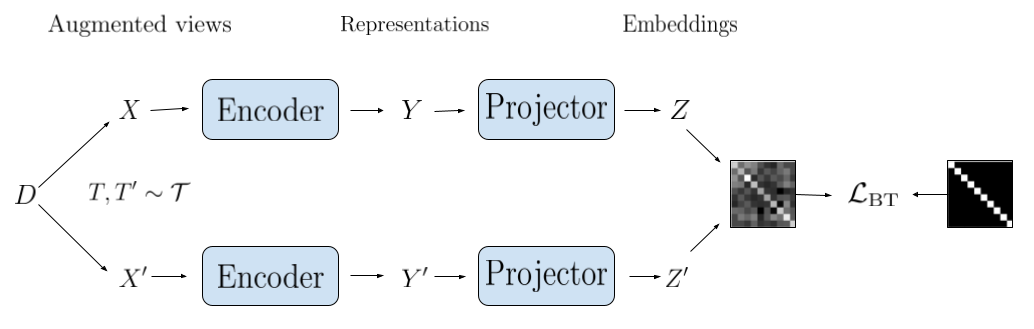
\includegraphics[scale=0.2]{BarlowTwins.png}
    \centering    
    \caption{\cite{zbontar2021barlow}}
\end{figure}

The loss function is calculated as the difference of the empirical cross-correlations of $Z_1$ and $Z_2$ is then calculated and the identiry matrix. 


\subsection{VIbCReg}
What is it?

VIbCReg \cite{lee2024vibcreg} is a non-contrastive SSL model based on VICReg \cite{bardes2022vicreg}. It has a joint embedding architecture,

How does it work?


\TODO{Ask Daeso if i can use image}
\begin{figure}[h]
    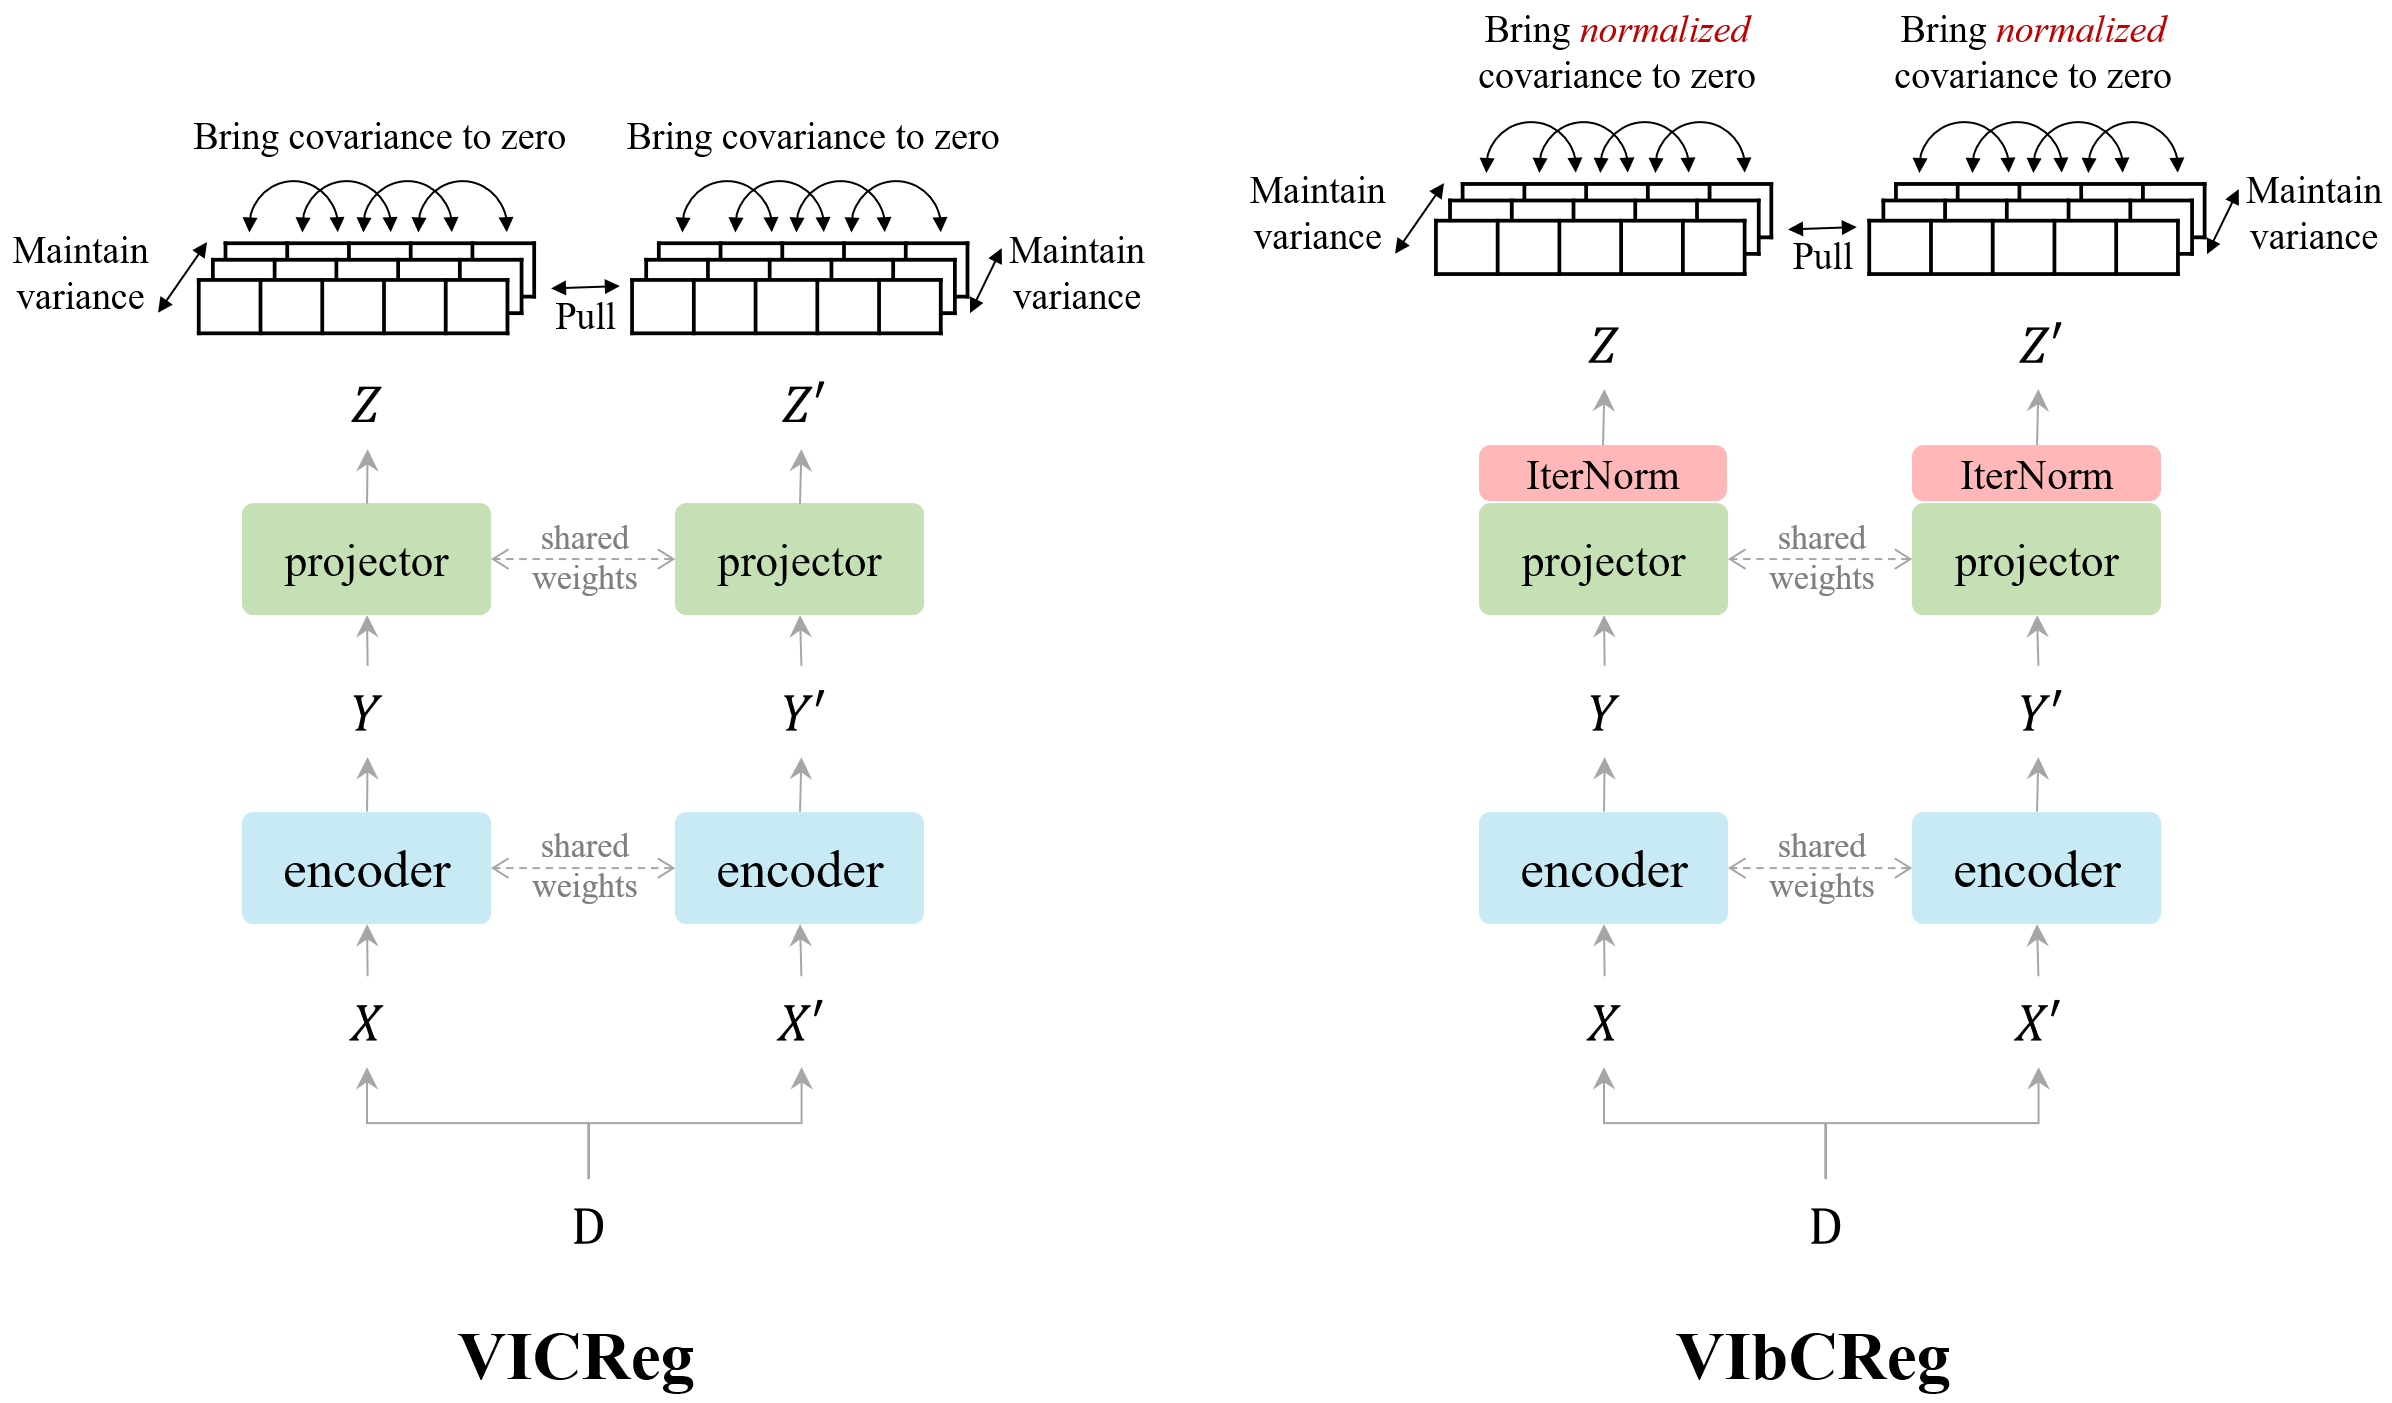
\includegraphics[scale=0.15]{VICReg_VIbCReg.png}
    \centering    
    \caption{\cite{lee2024vibcreg}}
\end{figure}



\section{Transformers}

When was it introduced, and by whom?
What lead up to its creation?
Why and where is it now widely used? 


Wiki: A deep learning architecture based on the multi-headed attention mechanism proposed in the 2017 paper "Attention is all you need".

One fo the main novelties of the architecture is not relying on recurrence, and instead solely using the attention mechanism to capture dependencies between input and output. As recurrent models are, in computational aspects, inherently sequential, there are major challanges when training as context windows, and sequence lengths become longer. 



\subsection{The attention mechanism}

\TODO{Wait for 3b1b video for context}

\begin{figure}[h]
    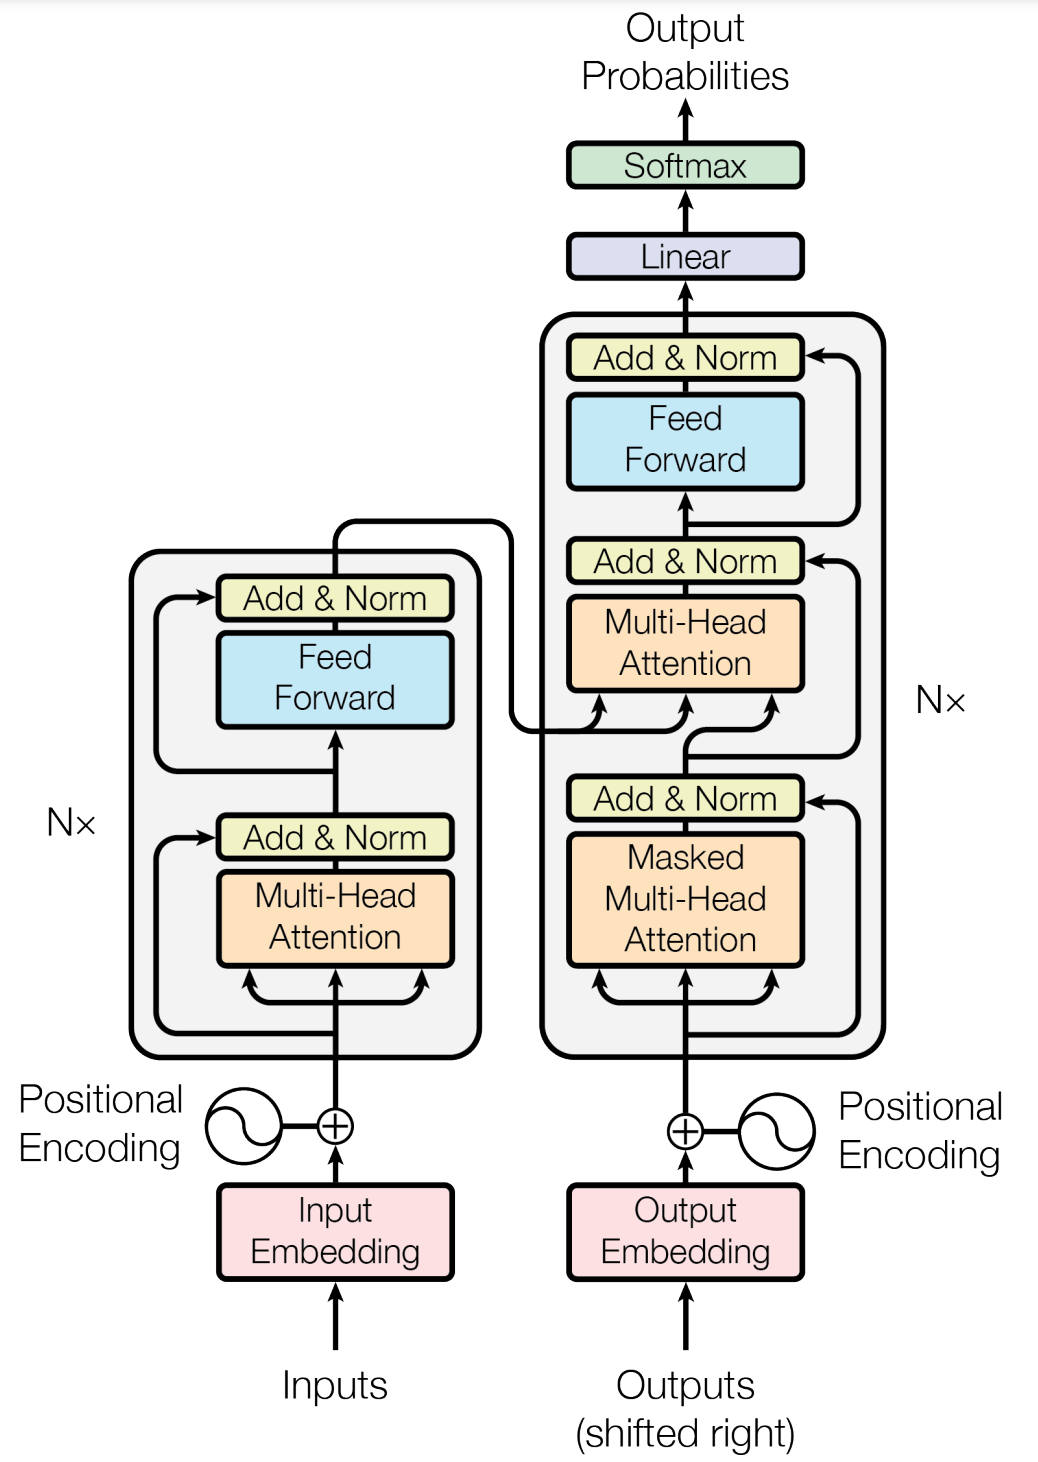
\includegraphics[scale=0.1]{Transformer_architecture}
    \centering    
\end{figure}

\subsection{Architecture}

Tokenizer

Positional encoding


Transformer layer (encoder/decoder)

\subsection{Bi-directional transformer (BERT)}

Unidirectional / 




\section{VQVAE}

\subsection{VAE}
Variational Autoencoders (VAE) is a family of latent variable models. 
\\\\

Dataset $X = \{x_i\}_{i=1}^{N}$ of iid samples (is this a nessecary assumption?). We assume that the data is a realization of some unobservable random process $Z$. This is to say that we assume there is a random variable $Z$ such that $x_i \sim p_{\theta}(x|z_i)$, where $z_i \sim p_{\theta}(z)$. As $Z$ is unobservable and the true distributions are unknown, one has to assume the form of the prior distribution $p_{\theta}(z)$ and the likelihood $p_{\theta}(x|z)$. Typically these are assumed to be Normal, as it allows for an array of numerical tricks to speed things up \todo{Reparameterization trick, etc, why do we use normal?}. As with any model where one wishes to employ gradient based learning, the distributions are assumed to be differentiable almost everywhere, both with respect to their parameters and argument. \\\\
VAEs have two components to their architecture. The first is an encoder, often called the inference model, $q_\phi(z|x)$ which approximates the true posterior. Secondly a decoder, often called the generative model $p_\theta(x|z)$, which approximates the likelihood. These models are typically parameterized by some type of neural network, and in that case $\phi$ and $\theta$ are the weights and biases of the two networks. 

\subsubsection{Training objective}

As with other variational methods, VAEs are optimized with respect to the \textit{evidence lower bound} or ELBO for short. Let $X$ and $Z$ be two jointly distributed variables, with distribution $p_\theta$. Then for any distribution $q_\phi$ the ELBO is defined as

\begin{equation}
    \begin{aligned}
        \label{eq:ELBO}
        \mathcal{L}_{\theta,\phi}(x) 
        &= \mathbb{E}_{q_\phi(z|x)} \log \left( \frac{p_\theta(x,z)}{q_\phi(z|x)}\right) \\ 
        &=  \mathbb{E}_{q_\phi(z|x)} \log \left( p_\theta(x)\right) + \mathbb{E}_{q_\phi(z|x)} \log \left( \frac{p_\theta(z|x)}{q_\phi(z|x)}\right) \\
        &= \log \left( p_\theta(x)\right) - \textrm{KL}(q_\phi(z|x)|| p_\theta(z|x)).
    \end{aligned}
\end{equation}

Due to the non-negativity of the KL-divergence, we see that the ELBO bounds the log likelihood of the data from below. By maximizing the ELBO with respect to the model parameters $\phi$ and $\theta$ one simultaneously maximizes the marginal likelihood, which improves the generative model, as well as reducing the KL-divergence of the approximate to the true posterior, which improves the inference model.



\begin{figure}[h]
    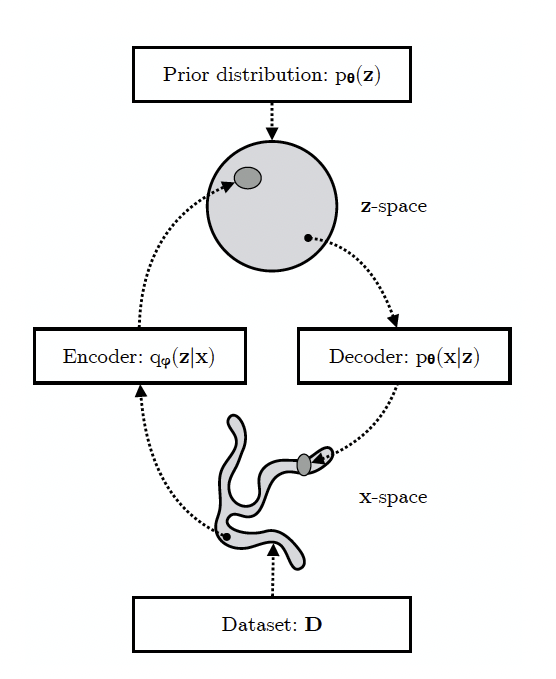
\includegraphics[scale=0.3]{VAE}
    \centering  
    \caption{\cite{VAE}, need to ask for premission or make own}  
\end{figure}

\subsection{VQVAE}
The Vector Quantized Variational AutoEncoder (VQ-VAE) was first introduced in \cite{VQVAE}. 

In contrast to VAEs, the prior and posterior is assumed to be categorical, as opposed to normal. 

Difference between VAE and VQ-VAE: 1. Maps input to discrete latent space insted of continious. 2. The prior, $p(z)$, is learned rather than static.

The posterior categorical distribution probabilities are defined as

\begin{equation}
    p(z=k | x) = 
    \begin{cases} 
        1 \quad \text{for }k = \textrm{argmin}_j||z_e(x) - e_j||_2 \\
        0 \quad \text{otherwise}
    \end{cases},
\end{equation}




\begin{figure}[h]
    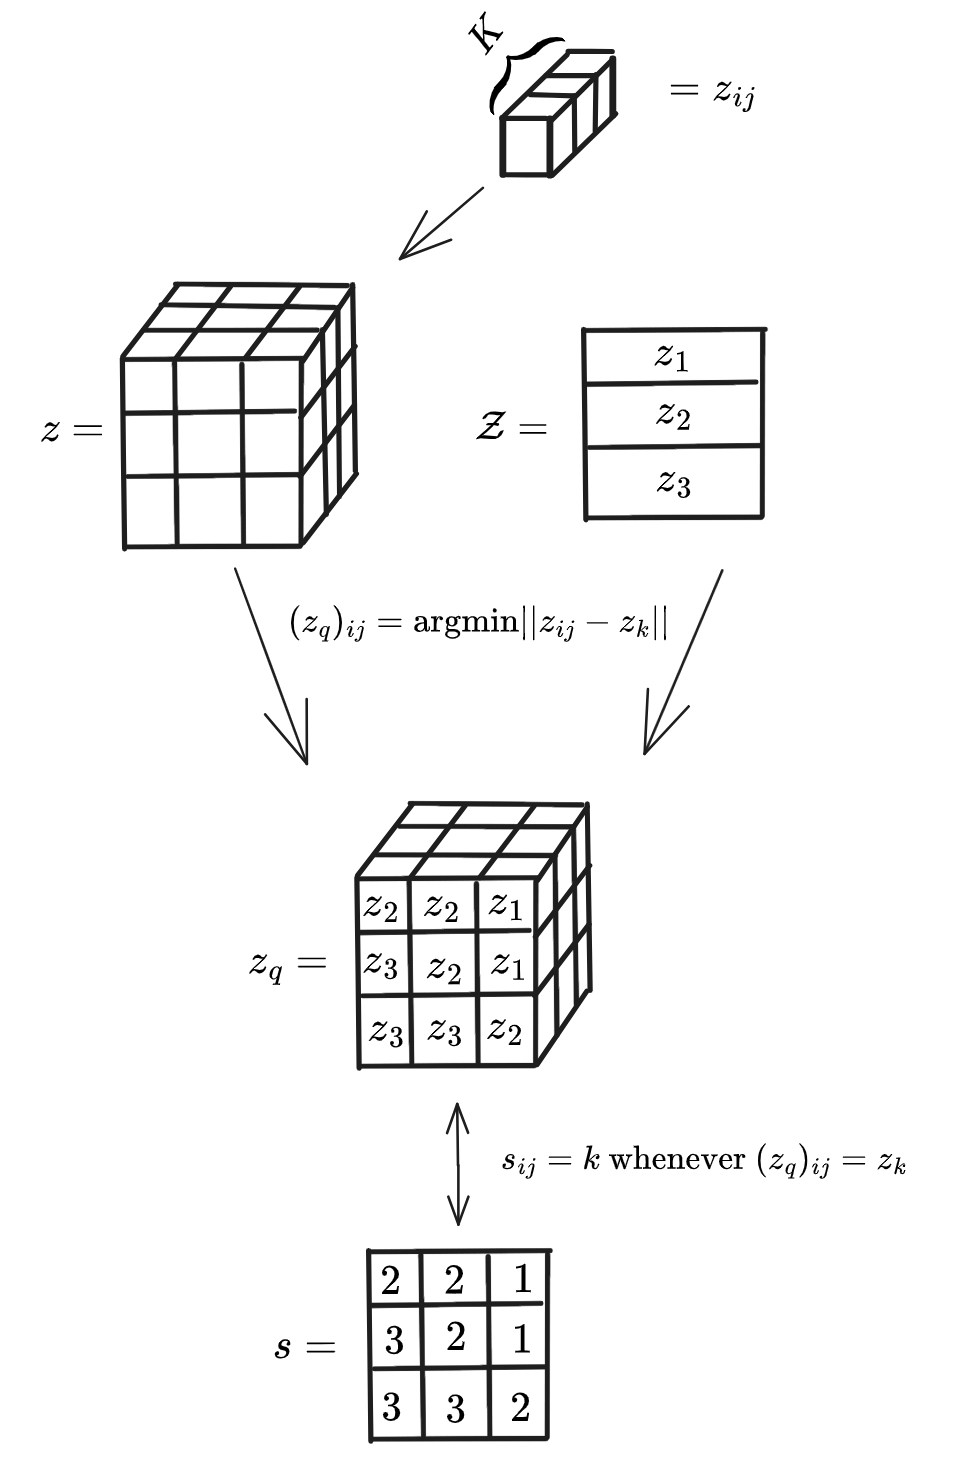
\includegraphics[scale=0.5]{quantization}
    \centering    
\end{figure}

\subsubsection{Codebook}

\subsubsection{Orthogonal regularization loss}

\cite{shin2023exploration} 

% \TODO{Reference https://github.com/lucidrains/vector-quantize-pytorch some way.}



\section{MaskGIT}

The Masked Generative Image Transformer is a generative transformer model for image synthesis developed by Google Research. The novelty of the model lies in the token generation. Unlike popular autoregressive generative transformers, who treat images as a sequence of tokens, MaskGIT introduces an image synthesis paradigm using a bi-directional transformer decoder. This means that during training MaskGIT learns to predict tokens in all directions, an intuitively more natural way to consider images. At inference time MaskGIT starts out with a blank canvas and predicts the entire image, and iteratively keeps and conditions on the most confident pixels.\\\\

\TODO{Intuitive introduction of masked modelling. Figures and such.}

The model assumes a tokenization procedure for stage 1, and in the original paper they used VQGAN \cite{VQGAN}. As MaskGIT only focuses on improving stage 2, present only that part. 

\subsection{Prior learning}

Start out with a sequence $s$ (b,n) of codebook indeces corresponding to a discrete latent representation $z_q$. Determine the proportion of tokens to mask according to the mask scheduling function $\gamma(t)\in (0,1]$. 
Sample a random subset of $s$ and replace values by [MASK] token in order to create the masked sequence $s_M$ (b,n). By a forward pass of the bi-directional transformer with $s_M$ as input obtain unnormalized logits (b,n,K), defining a distribution over the codebook indeces at each element. Calculate the loss as the binary cross-entropy of the logits and $s$. 

\subsection{Iterative decoding}

The bi-directional transformer could in principle predict all [MASK] tokens and generate a sample in a single pass by simply sampling from the logits obtained from a forward pass of an all masked sequence. However, there are challenges with this approach. In their original article \todo{spør om siteringsstil, og fiks denne setningen} \cite{chang2022maskgit} proposes a novel non-autoregressive decoding method to sythesize samples in a constant number of steps.\\\\

The decoding process goes from $t = 0$ to $T$. To genereate a sample at inference time one starts out with a all masked sequence which we denote by $s_M^{(0)}$. At iteration $t$ the model predicts the probabilities for all the [MASK] tokens, $p(\hat{s}_{ij}^{(t)}|s_M^{(t)})$, in parallell. Then at each masked entry $ij$ we sample a token index based on its predicted distribution.  

\subsection{Masking design}

For image generation, cosine schedulig function proved best across all experiments in the original paper. Start out by selecing just a few 


\end{document}